
Slike za učenje modela na početku smo pretvorili u CIELAB prostor boja. Generator za zadanu crno-bijelu sliku (L komponentu originalne obojene slike) treba generirati komponente A i B.
Na temelju generiranih A i B komponenti, stvara se obojena slika u CIELAB prostoru boja koja se prosljeđuje diskriminatoru.

Model smo učili 200 epoha. Za gubitak diskriminatora koristili gubitak unakrsne entropije, a za gubitak generatora koristili smo gubitak diskriminatora, kao i rekonstrukcijski gubitak (L1 udaljenost između umjetne i stvarne slike). Kao optimizator smo za obje mreže koristili optimizator Adam s početnom stopom učenja $2 \cdot 10^{-4}$ .
Nakon učenja modela, generator smo koristili za bojenje crno-bijelih slika. 

Usporedno su prikazane: crno-bijela slika,  slika obojena modelom cGAN i konačno stvarna slika u boji. Na slici \ref{fig:slike_skup} prikazan je izbor od nasumičnih 8 slika iz skupa COCO 2017 koje je model vidio pri učenju. Osim ovoga, prikazan je i izbor od 8 nasumičnih slika iz privatnih galerija ili s interneta koje model nije vidio pri učenju, na slici \ref{fig:slike_vlastite}.

\begin{figure}[H]
    \centering
    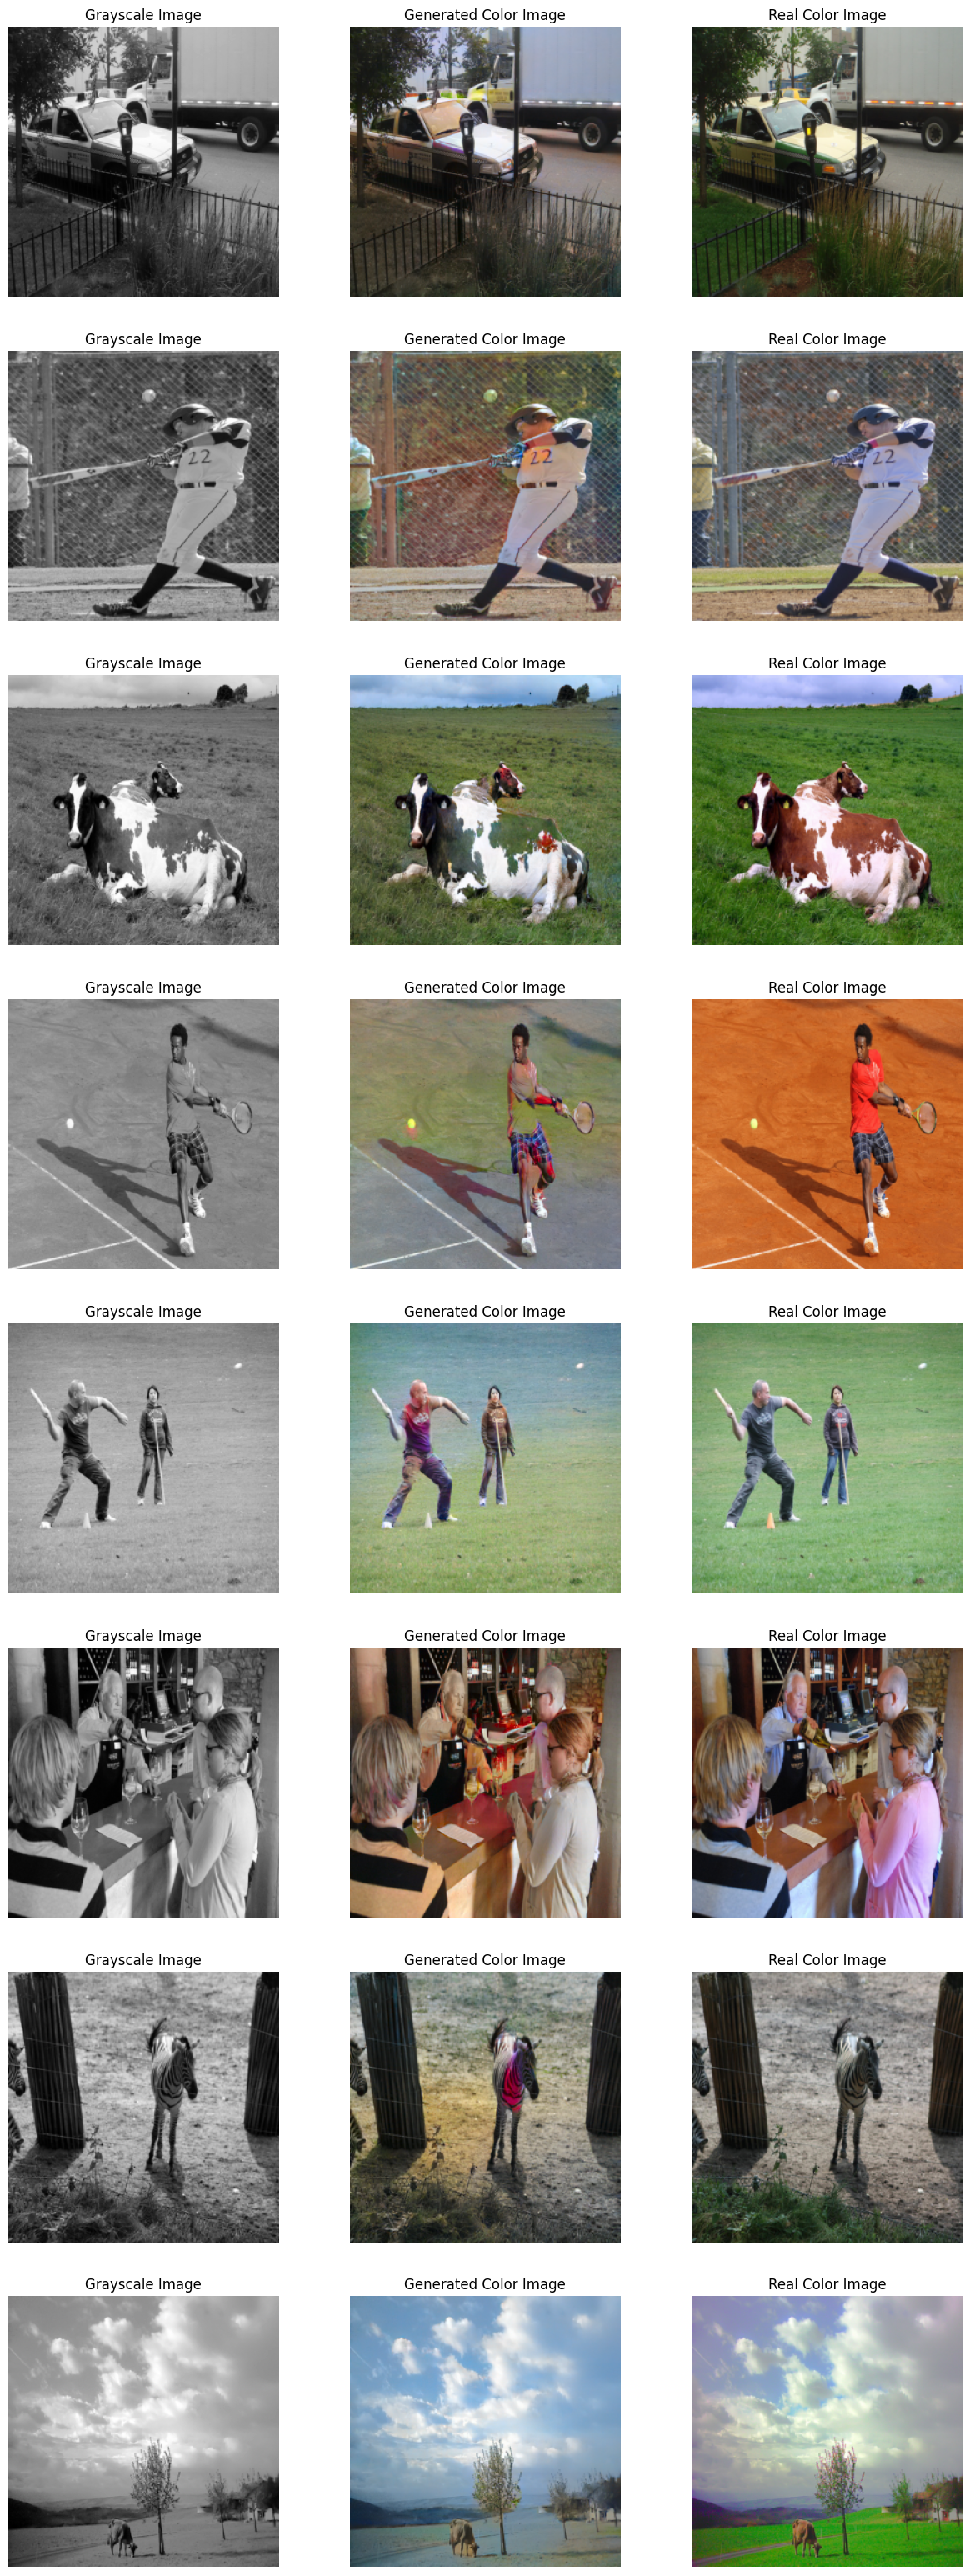
\includegraphics[width=0.9\linewidth]{imgs/slike_skup.png}
    \caption{Primjer obojenih slika iz skupa COCO 2017}
    \label{fig:slike_skup}
\end{figure}


\begin{figure}[H]
    \centering
    \includegraphics[width=0.9\linewidth]{imgs/slike_vlastite.png}
    \caption{Primjer obojenih vlastitih slika}
    \label{fig:slike_vlastite}
\end{figure}

Na temelju ovog uskog izbora slika, može se primijetiti da model mnogo bolje radi na slikama koje prikazuju prirodne scene i sadrže nijanse smeđe i zelene. Naš model dobro radi i na ljudskoj koži. Ovo možemo pripisati skupu podataka na kojemu je model učen - COCO 2017 sadrži velik broj slika na kojima su prikazani ljudi, kao i prirodne scene.

Osim provjere kvalitete obojenja ljudskim okom (koja je u ovakvom slučaju vrlo dobra mjera), potrebno je primijeniti objektivne matematičke mjere na izlaz modela. Korištene su, ranije spomenute, mjere IS (engl. \textit{Inception Score}) i FID (engl. \textit{Fréchet Inception Distance}). Rezultati su prikazani u tablici \ref{table:model_mjere}.

\begin{table}[H]
    \centering
    \caption{Mjere dobrote modela}
    \label{table:model_mjere}
    \begin{tabular}{ |c|c|c|c|c| }
        \hline
          \multicolumn{2}{|c|}{stvarne slike} & \multicolumn{2}{|c|}{obojene slike} &  \\
        \hline
        IS $\mu$ & IS $\sigma$ & IS $\mu$ & IS $\sigma$ & FID \\
        \hline
        5.2293 & 1.2776 & 5.1197 & 1.2776 & 8.5348 \\
        \hline
    \end{tabular}
\end{table}

Za stvarne slike dobivena je mjera IS iznosa $5.2293$ sa standardnom devijacijom od $1.2776$. Za obojene slike mjera IS iznosi $5.1197$ sa standardnom devijacijom od $1.2776$. Kada govorimo o zadatku bojenja slika, cilj je da je mjera IS što sličnija za obojene slike i stvarne slike. Dodatno, bolje je da je mjera veća uz što manju standardnu devijaciju - veći iznos mjere IS govori nam da su slike kvalitetne i raznovrsne. Ovaj model ima malu razliku između mjere IS za stvarne slike i obojene slike, svega $0.1096$. 

Za naš model, dobivena je mjera FID iznosa $8.5348$. Idealan iznos mjere FID je $0$ - ovo označava da ne postoji razlika u distribuciji stvarnih i generiranih tj obojenih slika. Koliko je ovo uspješno može se vidjeti tek usporedbom s nekim drugim modelima.